%%%%%%%%%%%%%%%%%%%%%%%%%% lecture-2
%\begin{frame}
%  \frametitle{lecture-2 算法---程序的灵魂}
%  \tableofcontents[hideallsubsections]
%\end{frame}

\section{数据类型}

\begin{frame}{基本数据类型}
\begin{itemize}
	\item 整数\lstinline|int|
	\item 单精度浮点数\lstinline|float|
	\item 双精度浮点数\lstinline|double|
	\item 字符\lstinline|char|
\end{itemize}
\textcolor{red}{机内用二进制表示, 不同数据类型占用存储空间大小不同。}
\end{frame}

\begin{frame}[fragile]{变量在使用之前首先要定义它的数据类型}
\begin{lstlisting}
#include<stdio.h>            // standard input/output编译预处理指令
int main()                   // 主函数
{                            // 函数开始标志
	int a,b;  // 定义变量a, b为整型数值,同类型变量可以在一条语句中定义。
	float f;  // 定义变量f为单精度浮点数
	double d; // 定义变量d为双精度浮点数
	char c;   // 定义变量c为单个英文字母
	a=10;	  // 变量赋值
	b=20;
	f=10.2;
	d=20.3;
	c='A';	  // 字符用单引号括起来
	return 0;                // 函数执行完毕返回函数值0
}                            // 函数结束标志
\end{lstlisting}
\end{frame}

\begin{frame}[fragile]{标识符}
标识符就是一个对象的名字。用于标识变量、符号常量、函数、数组、类型等。\\
\textcolor{blue}{以字母或下划线开始; 区分大小写; 不能使用关键字; 最好有含义。}
\begin{lstlisting}
#include<stdio.h>           
int main()                   
{                            
	int r = 123; // 合法整型变量名
	int 3a; // 不合法的变量名
	int break; // 不合法的变量名, 因为break是关键字, 被系统使用。
	int Radius; // 变量名最好有含义
	int radius; // 与Radius是不同的变量,C语言是到小写敏感的语言
	return 0;           
}                            
\end{lstlisting}
\end{frame}

\begin{frame}{C语言关键字}
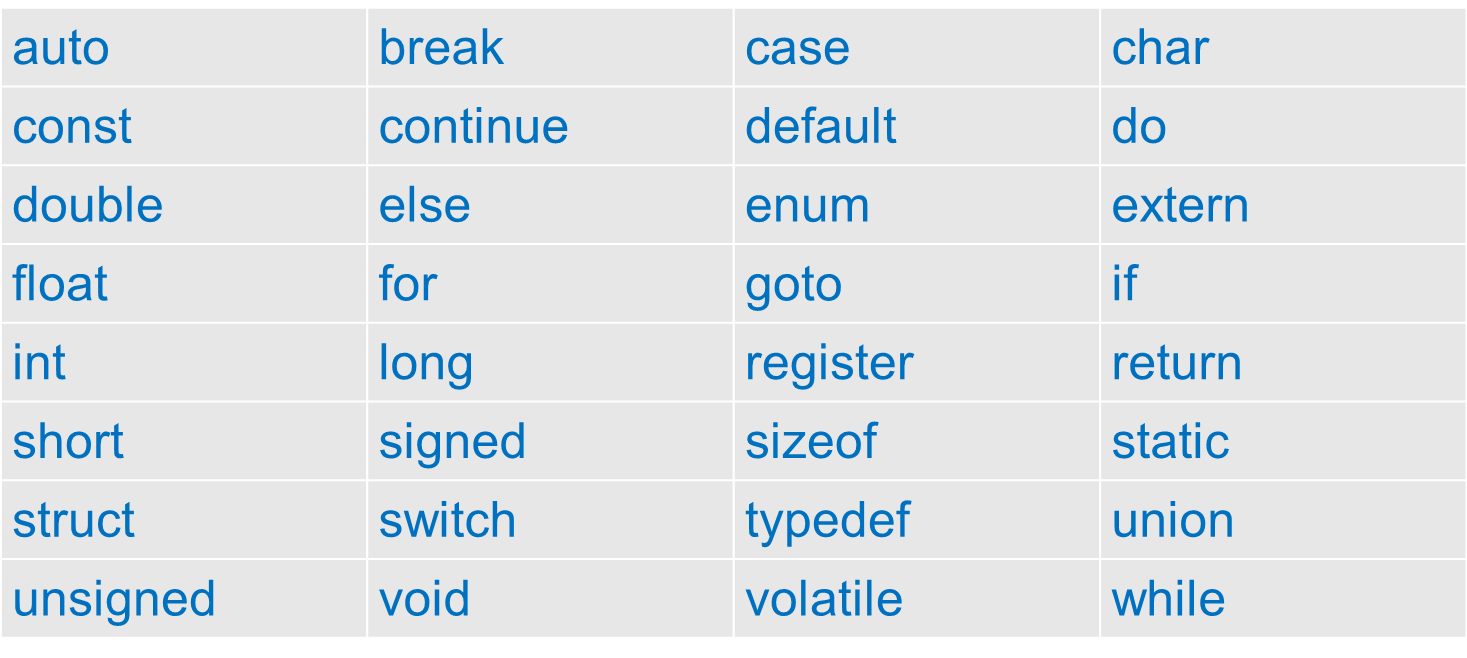
\includegraphics[scale=0.5]{key}
\end{frame}

\begin{frame}[shrink,fragile]{输出语句printf(``原样输出, \%格式符'', 对应变量值);}
\begin{lstlisting}
#include<stdio.h>            // standard input/output编译预处理指令
int main()                   // 主函数
{                            // 函数开始标志
	int a=10,b;    // 定义变量a, b为整型数值, 定义变量时,可以指定变量的初值
	float f=10.2;  // 定义变量f为单精度浮点数
	double d; // 定义变量d为双精度浮点数
	char c;   // 定义变量c为单个英文字母
	f=10.2;
	d=20.356;
	c='A';
	printf("a=%d,b=%d,c=%c,f=%f,d=%.2lf\n",a,b,c,f,d); // %.2f, %.2lf保留两位小数, \n为换行符
	return 0;                // 函数执行完毕返回函数值0
}                            // 函数结束标志
\end{lstlisting}
\textcolor{blue}{变量b没有被赋值, 将是一个随机值。}
\end{frame}

\begin{frame}{常用格式描述符与数据类型的对应关系}
\begin{tabular}{|c|c|c|}
	\hline 
	\textbf{格式符} & \textbf{对应的数据类型} &  \textbf{备注}\\ 
	\hline 
	\%d & int &  \\ 
	\hline  
	\%f & float &  \\
	\hline
	\%c & char & \\ 
	\hline   
	\%lf & double & \\ 
	\hline 
	\%.2f & float & 保留两位小数, 四舍五入。不适用于scanf()。 \\ 
	\hline 
	\%.2lf & double & 保留两位小数, 四舍五入。不适用于scanf()。 \\ 
	\hline
	\hline   
	\%x & int & 十六进制显示 \\ 
	\hline 
	\%ld & long int &  \\ 
	\hline 
\end{tabular}
\newline
\newline
\textcolor{blue}{详见p73, 表3.6}
\end{frame}


\begin{frame}{十进制与二进制}
\vspace{-1cm}
\begin{align*}
&\textcolor{red}{\text{十进制: 以10为底的幂展开式:}}\\
&(123)_{10}=1\times 10^2+2\times 10^1+3\times 10^0; \\
&\textcolor{blue}{\text{自低到高各位数(除10取余至商为0): }3=123\%10,~2=123/10\%10=12\%10,}\\
&\textcolor{blue}{1=123/10/10\%10=1\%10}\\
&\textcolor{red}{\text{二进制: 以2为底的幂展开式:}}\\
&(77)_{10}=(0100\quad 1101)_{2}=0\times 2^7+1\times 2^6+0\times 2^5+0\times 2^4\\
&\qquad +1\times 2^3+1\times 2^2+0\times 2^1+1\times 2^0\\
&\textcolor{blue}{\text{自低到高各位数(除2取余至商为0): }1=77\%2,~0=77/2\%2=38\%2,}\\
&\textcolor{blue}{~1=77/2/2\%2=19\%2,~1=77/2/2/2\%2=9\%2,}\\
&~\textcolor{blue}{0=77/2/2/2/2/\%2=4\%2,~0=77/2/2/2/2/2/\%2=2\%2,\dots}\\
\end{align*}
\end{frame}

\begin{frame}[shrink]
\frametitle{10进制、2进制、16进制的幂展开式}
\vspace{-0.5cm}
\begin{align*}
(D)_{10}&=D_{n-1}\times 10^{n-1}+D_{n-2}\times 10^{n-2}+\cdots+D_{1}\times 10^{1}+D_{0}\times 10^{0}\\
&+D_{-1}\times 10^{-1}+D_{-2}\times 10^{-2}+\cdots+D_{-m+1}\times 10^{-m+1}+D_{-m}\times 10^{-m}\\
&\\
(B)_{2}&=B_{n-1}\times 2^{n-1}+B_{n-2}\times 2^{n-2}+\cdots+B_{1}\times 2^{1}+B_{0}\times 2^{0}\\
&+B_{-1}\times 2^{-1}+B_{-2}\times 2^{-2}+\cdots+B_{-m+1}\times 2^{-m+1}+B_{-m}\times 2^{-m}\\
&\\
(H)_{16}&=H_{n-1}\times 16^{n-1}+H_{n-2}\times 16^{n-2}+\cdots+H_{1}\times 16^{1}+H_{0}\times 16^{0}\\
&+H_{-1}\times 16^{-1}+H_{-2}\times 16^{-2}+\cdots+16_{-m+1}\times 16^{-m+1}+H_{-m}\times 16^{-m}
\end{align*}
\end{frame}

\begin{frame}{进制对照表$2^32^22^12^0=8+4+2+1$}
\centering
\begin{tabular}{|>{\columncolor{yellow}}c|c|c||>{\columncolor{yellow}}c|c|c|}
\hline 
十进制 & 二进制 & 十六进制 & 十进制 & 二进制 & 十六进制 \\ 
\hline 
0 & 0000 &  0 & 8 & 1000  & 8 \\ 
\hline 
1 & 0001 &  1 & 9 & 1001  & 9 \\ 
\hline 
2 & 0010 &  2 & 10 & 1010  & A \\ 
\hline 
3 & 0011 &  3 & 11 & 1011  & B \\ 
\hline 
4 & 0100 &  4 & 12 & 1100  & C \\ 
\hline 
5 & 0101 &  5 & 13 & 1101  & D \\ 
\hline 
6 & 0110 &  6 & 14 & 1110  & E \\ 
\hline 
7 & 0111 &  7 & 15 & 1111  & F \\ 
\hline 
\end{tabular} 
\end{frame}

\begin{frame}{十进制、二进制与十六进制举例}
\vspace{-0.5cm}
\begin{align*}
(123)_{10}&=1\times 10^2+2\times 10^1+3\times 10^0; \\
&\textcolor{blue}{\text{自低到高各位数: }3=123\%10,~2=123/10\%10,~1=123/10/10\%10}\\
&\\
(77)_{10}&=(0100\quad 1101)_{2}=0\times 2^7+1\times 2^6+0\times 2^5+0\times 2^4\\
&+1\times 2^3+1\times 2^2+0\times 2^1+1\times 2^0\\
&\\
(77)_{10}&=(4D)_{16}=4\times 16^1+13\times 16^0
\end{align*}
\end{frame}

\begin{frame}[shrink]{数值在计算机中的表示(以8bit编码为例)}
\begin{itemize}
	\item 原码:正数的符号为0,负数的符号为1,其它位按一般的方法表示数的绝对值。
	\vspace{-0.5cm}
	\begin{align*}
	x=(+103)_{10}  &&[x]_{\text{原}}=(\textcolor{red}{0}1100111)_{2}\\
	x=(-103)_{10}  &&[x]_{\text{原}}=(\textcolor{red}{1}1100111)_{2}
	\end{align*}
	\item 反码: 正数的反码与原码相同;负数的反码是符号位不变,其他位按位取反 
	\item 补码: 正数的补码与其原码相同;负数的补码为其反码最末位加1. 即,
	
	\textcolor{blue}{负数补码 = 反码$+1=2^n-$该数的绝对值, $n$是编码二进制位数.}
\end{itemize}
\vspace{-0.5cm}
\begin{align*}
(77)_{10}&=(\textcolor{red}{0}100\quad 1101)_{2},\qquad (-77)_{10}=(\textcolor{red}{1}100\quad 1101)_{2}\\
(-77)_{\text{补}}=2^8-77&=\textcolor{red}{1}111\quad 1111 +\textcolor{red}{0}000\quad 0001 - \textcolor{red}{0}100\quad 1101\\
&=\underbrace{\textcolor{red}{1}111\quad 1111 - \textcolor{red}{0}100\quad 1101}_{(-77)_{\text{反}}} + ~\textcolor{red}{0}000\quad 0001\\
&=\underbrace{\textcolor{red}{1}011\quad 0010 }_{(-77)_{\text{反}}}+ \textcolor{red}{0}000\quad 0001=1011\quad 0011
\end{align*}
\end{frame}

\begin{frame}{数值表示示例}
\centering
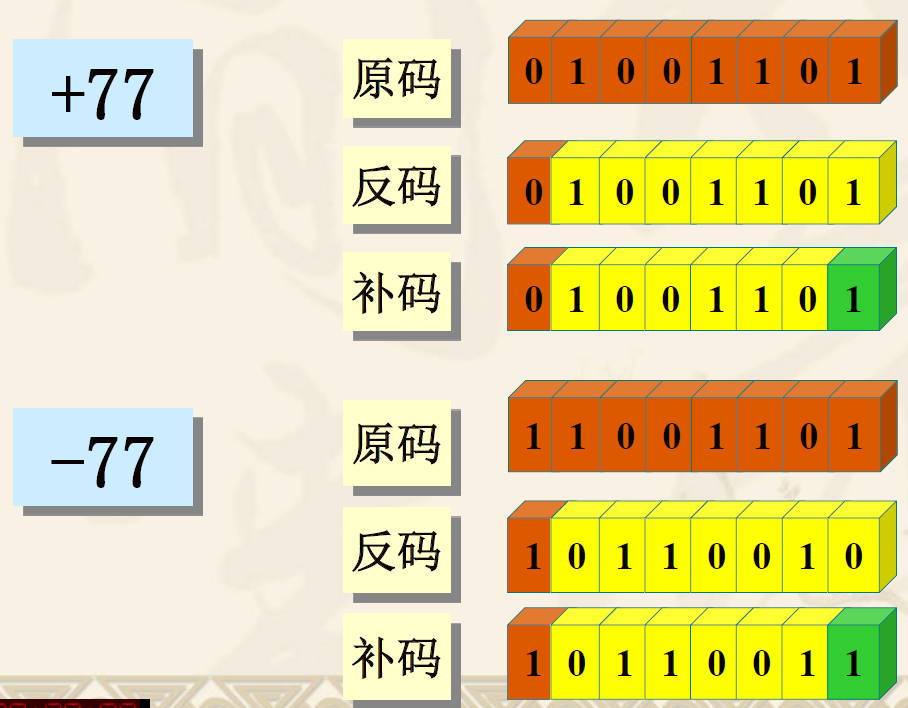
\includegraphics[scale=0.25]{2}
\end{frame}

\begin{frame}{机内以补码形式存储有符号数}
\begin{enumerate}
\setlength{\itemsep}{.5cm}
\item 对于正数,原码=反码=补码
\item 对于负数,补码=反码 + 1\\
反码 = 符号位不变, 其他位按位取反
\item 补码是可逆的,即再对补码求补得到原码。
\item 引入补码后,使减法统一为加法。
$(+77)_{\text{补}}+(-77)_{\text{补}}=0100~1101+1011~0011=0000~0000$	
\end{enumerate}
\end{frame}

\note
{
0原码是00000000 -0原码是10000000

0反码是00000000 -0反码是11111111

0补码是00000000 补码没有正0与负0之分。+0和-0的补码是一样的。即 0的补码只有一种表示。

+0的补码:00000000

-0的补码:第一步:11111111 第二步+1= 1 00000000 第三部:进位1被丢弃 您明白了吗?

在规定中,8位二进制码能表示的反码范围是-127~127。

此时(字长为8位), -128没有原码和反码(只有补码)。

那么,为什么规定字长8位时-128没有原码和反码呢?下面解释。

首先看-0,[-0]原码=1000 000,其中1是符号位,求反操作,算出[-0]反码=1111 1111,

再看-128,假如它有原码且[-128]原码=1000~000,假如让-128也有反码,求反操作,则[-128]反码=1111~1111,

你会发现,-128的反码和-0的反码相同,所以为了避免面混淆,有了-0的原码,便不能有-128的原码补码,这是8位比特位位数限制决定的。
}

\begin{frame}{补码运算实例(以8bit编码为例)}
\textcolor{blue}{补码可逆:}
\begin{align*}
&[-25]_{\text{原}}=(1001~1001)_2\quad [-25]_{\text{反}}=(1110~0110)_2\\
&[-25]_{\text{补}}=[-25]_{\text{反}}+1=(1110~0110+1)_2=(1110~0111)_2\\
&[-25]_{\text{原}}=\left([-25]_{\text{补}}\right)_{\text{补}}=(1001~1000+1)_2=(1001~1001)_2
\end{align*}

\textcolor{blue}{减法统一为加法: $[a-b]_{\text{补}}=a_{\text{补}}+[-b]_{\text{补}}$}
\begin{align*}
&[102-25]_{\text{补}}=[77]_{\text{补}}=(0100~1101)_2=77\\
&[102]_{\text{补}}+[-25]_{\text{补}}=(0110~0110)_2+(1110~0111)_2=(0100~1101)_2=77\\
&\text{所以, }[102-25]_{\text{补}}=[102]_{\text{补}}+[-25]_{\text{补}}\\
&\text{同样有, }[25-102]_{\text{补}}=[25]_{\text{补}}+[-102]_{\text{补}}\\
\end{align*}
\end{frame}

\begin{frame}{计算机数据存储单位}
位(bit)是最小的存储单位,每一位存储1位二进制码, 一个字节(Byte)由8位组成。
\begin{itemize}
	\item 1B = 8b
	\item 1KB = 1024B
	\item 1MB = 1024KB
	\item 1GB = 1024MB
	\item 1TB = 1024GB
\end{itemize}
\end{frame}

\note{ 1B = $2^3$b (8位), 1KB = $2\times 2^8$ = $2^10$ B}

\begin{frame}[shrink,fragile]{整型数据输出printf(``\%d,\%x'', -25, -25);}
\begin{lstlisting}
#include<stdio.h>            // standard input/output编译预处理指令
int main()                   
{                            
	int a=-25,b=102;    // 定义变量a, b为整型数值, 定义变量时,可以指定变量的初值
	
	printf("a=%d,b=%d,a=%x,b=%x\n",a,b,a,b); 
	printf("%d,%d,%x,%x\n",-25,-25,102,102); 
	printf("%d,%d,%x,%x,%X\n", 77,-77,77,-77,-77);
	// 编译运行, 解释输出结果。
	return 0;                
}                            
\end{lstlisting}
\end{frame}

\begin{frame}{ASCII编码表$B_6B_5B_4B_3B_2B_1B_0$}
\begin{columns}
	\column{0.65\textwidth}
	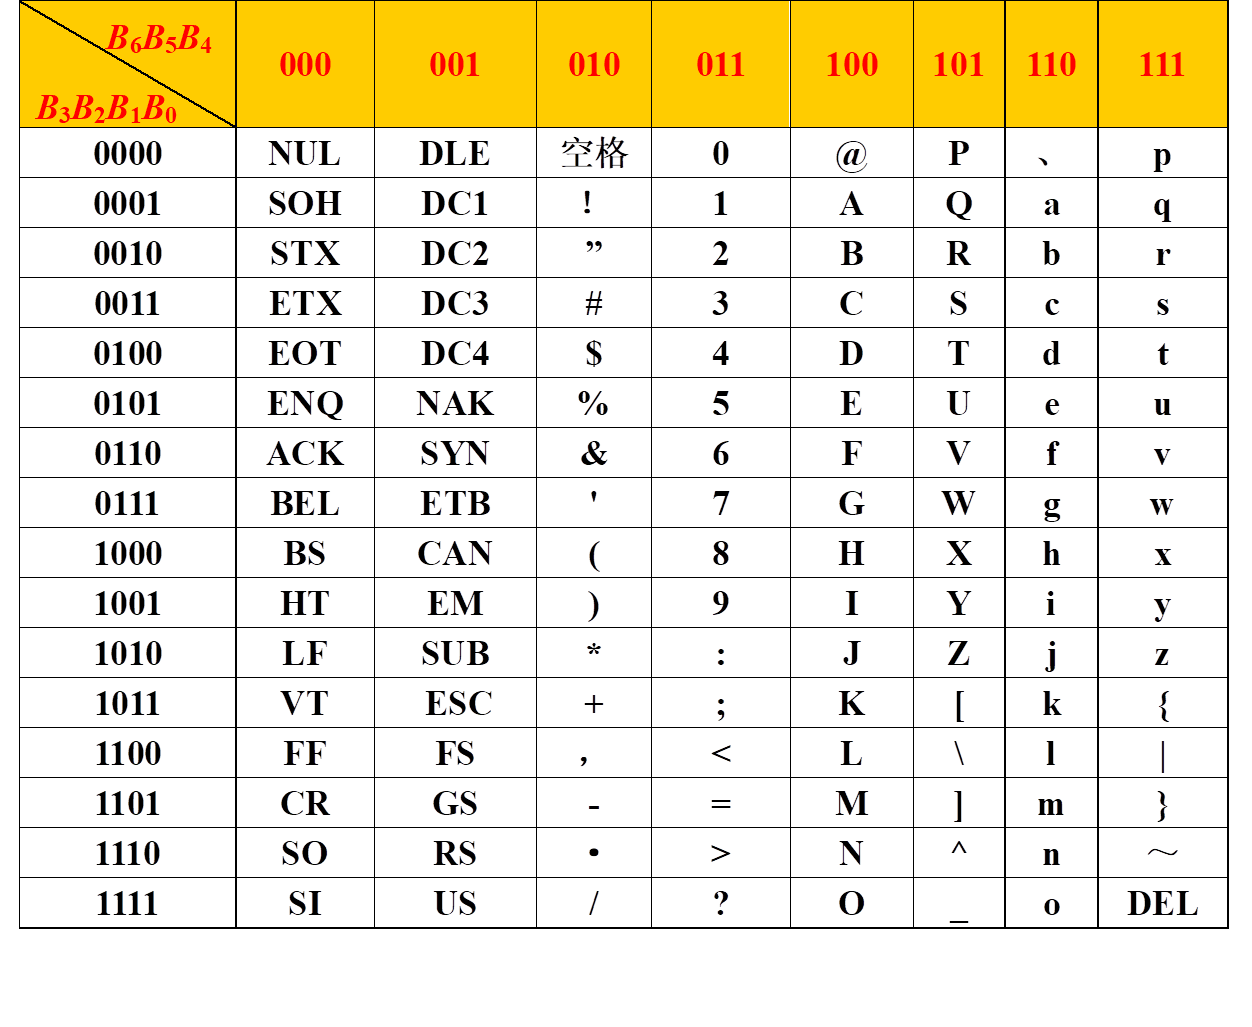
\includegraphics[scale=0.4]{ASCII}
	\column{0.35\textwidth}
	\begin{itemize}
		\item ASCII码连续排列 \\
		`0'$\sim$`9', `A'$\sim$`Z', `a'$\sim$`z'
		\item 数字 = 编码值 - `0' \\
		9=`9'-`0'
		\item 大小字符间隔: \\
		`a' - `A' = 32
		
		\scriptsize{
			`a'=0110~0001=61H=0X61=97
			
			'A'=0100~0001=41H=0X41=65}
	\end{itemize}	
\end{columns}
\end{frame}

\begin{frame}[shrink,fragile]{字符类型}
\begin{lstlisting}
#include<stdio.h>           
int main()                   
{                            
	char c1 = 'A', c2 = 'a', c3 = '\n'; // 字符型变量
	printf("%c,%c,%d\n",c1,c2,c3); // A,a,10
	// 整型变量的整数值就是ASCII编码值
	printf("%c,0X%x,%d\n",c1,c1,c1); // A,0X41,65
	c1 = c1 + 1; // 在表达式中, char类型看作int处理
	printf("%c,0X%x,%d\n",c1,c1,c1); // B,0X42,66
	c1 = c1 + 32;  // 转换为小写字母
	printf("%c,0X%x,%d\n",c1,c1,c1); // b,0X62,98
	printf("%d\n",'9'-'0'); // 数字 = 编码值- '0'
	printf("%c,%d,%c,%d\n",'A','A','a','a'); // 输出字符和相应的ASIII编码
	return 0;           
}                            
\end{lstlisting}
\end{frame}


\begin{frame}[shrink,fragile]{常量}
\vspace{-0.2cm}
\begin{lstlisting}
#include<stdio.h> 
#define PI 3.14  // 符号常量, 注意没有分号           
int main()                   
{                                  
	int a = 123; // 整型常量
	float f = 12.2, f1=123E-1; // 实型常量
	char c1 = 'A', c2='\n'; // 字符常量
	char s[50] = "boy"; // 字符串常量
	printf("半径为%d的圆周长是%f\n",a,2*PI*a);       
	printf("回车换行\n");
	printf("单引号\',双引号\"转义字符前缀\,\n");  
	return 0;           
}                            
\end{lstlisting}
\textcolor{blue}{转义字符, 见p40, 表3.1}
\end{frame}

\begin{frame}[fragile]{常量与常变量}
\begin{lstlisting}
#include<stdio.h> 
#define PI 3.14  // 符号常量, 注意没有分号           
int main()                   
{                            
	int r = 123; // 整型变量
	const int a = 425; // 常变量
	r = 100; // 合法, 因为r是变量,可以随时更改它的值
	a = 100; // 不合法,因为a是常变量,不能更改
	printf("半径为%d的圆周长是%f\n",r,2*PI*r); 
	return 0;           
}                            
\end{lstlisting}
\end{frame}

\begin{frame}[fragile,shrink]{长整型、无符号整型, 浮点型数据类型}
\begin{lstlisting}
#include<stdio.h>           
int main()                   
{                            
	int a = 123; // 整型变量
	long int b = 1E+8; // 长整型变量
	unsigned int u = 0XFF; // 无符号整型, 最高为不作为符号位处理
	float f = 10.2; // 单精度浮点数
	double d = 1E-8; // 双精度浮点数
	printf("%x,%d\n",u,u); // ff, 255
	printf("%d,%ld,%x,%f,%lf\n",a,b,u,f,d);
	// sizeof函数返回类型分配的字节数,整型数据存储空间和值的范围见p45, 表3.2
	printf("%d,%d,%d,%d\n",sizeof(int),sizeof(float),sizeof(double),sizeof(long int),sizeof(long long int));
	return 0;           
}                            
\end{lstlisting}
\end{frame}



